
\documentclass{beamer}
\mode<presentation>
\usepackage{amsmath}
\usepackage{amssymb}
%\usepackage{advdate}
\usepackage{graphicx}
\graphicspath{{../figs/}}
\usepackage{adjustbox}
\usepackage{subcaption}
\usepackage{enumitem}
\usepackage{multicol}
\usepackage{mathtools}
\usepackage{listings}
\usepackage{url}
\def\UrlBreaks{\do\/\do-}
\usetheme{Boadilla}
\usecolortheme{lily}
\setbeamertemplate{footline}
{
  \leavevmode%
  \hbox{%
  \begin{beamercolorbox}[wd=\paperwidth,ht=2.25ex,dp=1ex,right]{author in head/foot}%
    \insertframenumber{} / \inserttotalframenumber\hspace*{2ex} 
  \end{beamercolorbox}}%
  \vskip0pt%
}
\setbeamertemplate{navigation symbols}{}
\let\solution\relax
\usepackage{gvv}
\lstset{
%language=C,
frame=single, 
breaklines=true,
columns=fullflexible
}

\numberwithin{equation}{section}
\title{9.2.34}
\author{AI25BTECH11001 - ABHISEK MOHAPATRA}
% \maketitle
% \newpage
% \bigskip
\begin{document}
{\let\newpage\relax\maketitle}
\renewcommand{\thefigure}{\theenumi}
\renewcommand{\thetable}{\theenumi}






	 	\textbf{Question}:
Find the area of region bounded by the line $x = 2$ and the parabola $y^2 = 8x$.

		\textbf{Solution:}

	Graph:
\begin{figure}[h!]
	\centering
	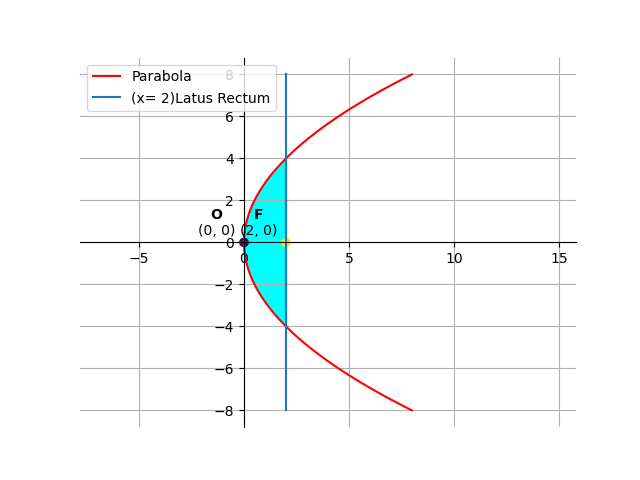
\includegraphics[width=0.7\linewidth]{img.png}
\end{figure}

From the given information, the parameters of the parabola and line are
\begin{align}
		\vec{V} = \myvec{0&0\\0&1}, \vec{u} = \myvec{-4\\0} , f = 0, \vec{h} =\myvec{2\\0}, \vec{m}=\myvec{0\\1} 
\end{align}
Substituting from the above in (9.1.1.3),
\begin{align}
k_i=4,-4
\end{align}
yilelding the points of intersection
\begin{align}
		\vec{a_0}=\myvec{2\\4},\vec{a_1}=\myvec{2\\-4}
\end{align}
Thus, the area of the parabola in between the lines $x = 2$ is given by
\begin{align}
\int_0^2 \sqrt{8x} = \frac{16}{3}
\end{align}


\end{document}




